\documentclass{report}
\usepackage[utf8]{inputenc}
\usepackage{fullpage}
\usepackage{graphicx}
\usepackage{booktabs}
\title{LINGI2146 - Project - Attacks against RPL}
\author{Nicolas Houtain \& Nicolas Gorby Kabasele \& Arthur Paquot}
\renewcommand{\thesection}{\arabic{section}}

\begin{document}
\maketitle
\section{Introduction}
We choose as our subject for this project the attacks against the RPL protocol. Nowadays, the internet of thing gains more and more interest and RPL could be one of the protocol used for those low power and lossy networks. We were interested to see if this protocol was robust enough to avoid an attack to corrupt the network. In order to do so, we selected a few known attacks for those kind of network and we try to implement them in Contiki and simulate the behavior of the network with Cooja. The different attacks that we present are a sinkhole attack, a select-forwarding attack, a version number attack and DAG inconsistency attack. For each attack we briefly present the attack, how we implemented it and how the network and the RPL protocol react to those attacks. For all the attack, the malicious behavior can be activated by pressing the button of the mote.
\section{Sinkhole attack}
A sinkhole attack is when a node announces an artificial beneficial routing path. The other nodes of the network will therefore chose the malicious node as their parent and most of the traffic will pass by the malicious node.
\subsection*{Implementation}
We choose to implement the sinkhole attack by making the malicious node announcing a rank higher that its real one. The malicious node will advertise the rank 256 which the rank of the root. This is done in the [FILE.c] in the method [method].
\subsection*{Consequences on the network}
All the neighbor of the malicious node will chose it as their parent since they think it's the root of the graph. A lot of the traffic will therefore pass by the malicious node. This attack is powerful when coupled with other attacks. Indeed, since an important part of the traffic will pass by the malicious node, it has the opportunity to corrupt, drop or do anything other malicious action on the packets.
\subsection*{Countermeasure}

\subsection*{Measurement}
\begin{table}[h!]
	\centering
	\caption{Impact of  sinkhole on DAO MSG}
	\begin{tabular}{cccc}
		\toprule
		Type&DIO MSG & DAO MSG&time\\
		\midrule
		Non-malicious&31&1&2:30\\
		Malicious&31&25&2:30\\
		Non-malicious&35&1&3:45\\% A VERIFIER
		Malicious&35&30&3:45\\
		\bottomrule
	\end{tabular}
\end{table}
\section{Select-Forwarding Attack}
A select forwarding attack is an attack where a malicious node decides arbitrarily which packet it will forward and which packet it will drop. This kind of attack is really hard to detect for a protocol such as RPL since the RPL packet are still distributed in the network, but all the IPV6 packet for example, are dropped. The node that doesn't receive the packet can not notice that there is a bad behavior and the nodes that sent it can think the packet were lost. 
\subsection*{Implementation}
We choose to drop all the IPV6 packet that the malicious node received (packet that are not RPL packet). In order to do so, every time the malicious node receives a ping packet, it will consider that its header is wrong and will drop the packet. This is done in the \textit{ext-header.c} file in the method [NAME], where the node, if malicious, returns "-1".  [CE SERAIT MIEUX QU IL DROP PAS LES PACKETS QUI LUI SONT DESTINES]
\subsection*{Consequences on the network}
When the malicious node is activated, all the ping packet that has to reach a node to which the path pass by the malicious node are dropped. This kind of attack is really powerful if coupled with a sinkhole attack. In such case, most of the ping packet pass by the malicious node and are discarded. 
\subsection*{Countermeasures}
It is difficult for a network to notify that some packet are lost, especially with a protocol such as RPL where the lost of packet happens really often. We let our little network running for several minute to let RPL the time to spot the error, but no changes happen.

\subsection*{Measurement }
When the malicious behavior is not activated, every mote on the network can be pinged from the outside thanks to the \textit{ping6} command. However, when the mote becomes malicious, all the mote to which the path pass by the malicious node are not pingable anymore. We put a printf in the code to show when the malicious node drops the packet. 
\section{Version Number Attack}
In the RPL protocol, each DIO message has a version number that is incremented by the root each time a rebuilding of the DODAG is needed. If a node has a version number smaller than the one of the root, it means that the node has not migrated to the new DODAG and can therefore not be used as a parent. If an malicious node increase the version number of the DIO messages it sends, the other node will think that are not up to date and will rebuild the DODAG graph.

\subsection*{Implementation}
In order to perform that attack, the malicious node, every time it sends a DIO message, will increase the version number by one. This is done in the \textit{rpl-icmp6.c} file in the method \textit{dis\_output}.

\subsection*{Consequences on the network}
This attack has several consequences on the behavior of the network. It can creates loop in the network, leading to the lost of packets and all the successive and unnecessary rebuilding of the graph increase the traffic of packet in the network. This consume the availability of the links and the nodes that could be used for relevant traffic. This overhead can exhaust the resources of the node and lead to a congestion of the network. 
[PARLER DES TIMER]
\subsection*{Countermeasure}
A countermeasure for this attack could be a way to authenticate the version number, i.e., that it was modified by the root and not by an other node. With hash or cryptography mechanism, the version number of the DIO packet could be verified by a node, if the hash value doesn't correspond to the one expected, the version number is not taken into account. Note that such a verification system will consume more resources on the root, that has to use some mechanism to produce the version number and on the different nodes that have to check the correctness of the version number.
\subsection*{Measurement }
The consequence of the attack can be watched using the MPS stack viewer provided by Cooja. We can observe that the stack of the nodes surrounding the malicious one is much bigger when the attack has been launched. Indeed, the reset of the different timers increases the traffic of messages between the different nodes.\\

\begin{figure}
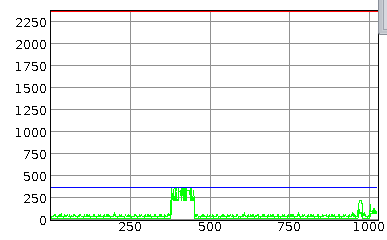
\includegraphics[scale=0.4]{img/normal_stack2}
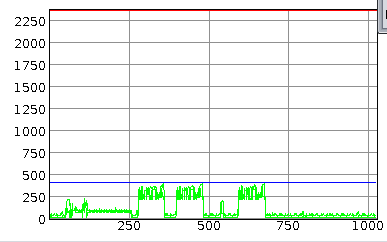
\includegraphics[scale=0.4]{img/normal_stack4}
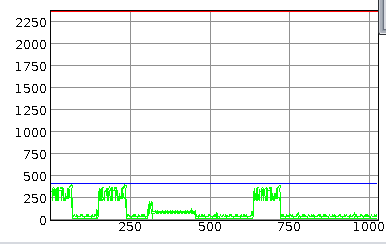
\includegraphics[scale=0.4]{img/normal_stack5}\\
\caption{Stack of a non-malicious node with no malicious node in the network}
\end{figure}

\begin{figure}
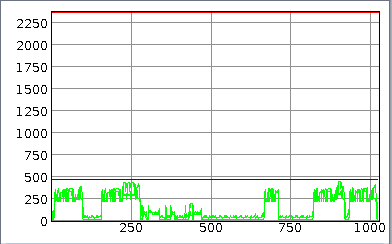
\includegraphics[scale=0.4]{img/mali_sta2}
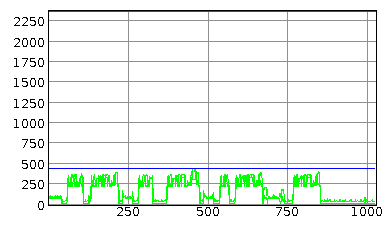
\includegraphics[scale=0.4]{img/mali_sta7}
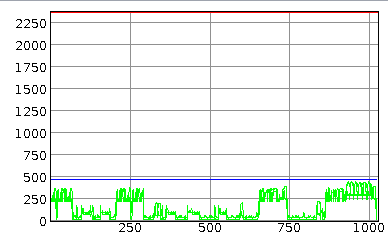
\includegraphics[scale=0.4]{img/mali_sta5}
\caption{Stack of a non-malicious with malicious node in the network}
\end{figure}

When the malicious node performs its attack, the stacks of the non-malicious nodes surrounding it are almost never still. On the other hand, when no malicious node is in the network, the stack can be still for several seconds, grows when some messages are exchanged and then becomes still again.\\

Moreover, we put a printf in the code to show when an inconsistency is found, this leads to the reset of the timer, responsible of the increase of teh traffic. The root also receives an DAG message with an inconsistent version and it reset its timer too, to rebuild the DODAG.
%\includegraphics[scale=0.5]{malicious_stack}
\section{DAG Inconsistency Attack}
A DAG inconsistency is when the packet doesn't follow the direction that matches the rank relationship. In that case, the node that notices the inconsistency, it uses the rank error bit flag to advertise that this packet is inconsistent. When a node receives an inconsistent packet with the rank error bit set, it reset the timer and drop the packet. A malicious node could therefore set the rank error bit of all the packet it receives, leading to the reset of the timer and the lost of packet.\\

Note that the opposite attack is also possible, the malicious node doesn't set the flag where a loop is detected. This attack is more difficult to implement since we have to create loop in the network to verify if the attack works, we therefore chose to implement the first version.

\subsection*{Implementation}
The RPL protocol implemented in Contiki doesn't drop the packet when the rank error bit is set. However, it could be some situations where we would prefer to drop a pack that is inconsistent, we therefore change the behavior of the RPL protocol to make it drop a packet when the rank error bit is set. The malicious node set the flag for all the packet it receives. This is done in the \textit{ext-header.c} file in the method [NAME].

\subsection*{Consequences on the network}
One of the immediate outcome of the attack is to reset the timer of the node that receives the packet. The node will therefore send DIO message more frequently, leading to an unnecessary used of the links and the battery. The different neighbor of the node are also victim of the attack since they have to process a useless traffic. Moreover, the node will drop the different packet it receives with the flag set.

\subsection*{Countermeasures}

One solution could be to limit the number of time a node can reset its timer during a lapse of time. 
\subsection*{Measurement}
The DAG inconsistency results in the lost of packets and the reset of the timers. The traffic is therefore increased.

\section{A NODE THAT JOINS AND LEAVE THE NETWORK ALL THE TIME}

\end{document}